% !TEX TS-program = pdflatex
% !TEX encoding = UTF-8 Unicode

% This is a simple template for a LaTeX document using the "article" class.
% See "book", "report", "letter" for other types of document.

\documentclass[11pt]{article} % use larger type; default would be 10pt

\usepackage[utf8]{inputenc}
\usepackage[T1]{fontenc}
\usepackage[magyar]{babel}

%%% Examples of Article customizations
% These packages are optional, depending whether you want the features they provide.
% See the LaTeX Companion or other references for full information.

%%% PAGE DIMENSIONS
\usepackage{geometry} % to change the page dimensions
\geometry{a4paper} % or letterpaper (US) or a5paper or....
\geometry{margin=3cm} % for example, change the margins to 2 inches all round
% \geometry{landscape} % set up the page for landscape
%   read geometry.pdf for detailed page layout information

\usepackage{graphicx} % support the \includegraphics command and options

% \usepackage[parfill]{parskip} % Activate to begin paragraphs with an empty line rather than an indent

%%% PACKAGES
\usepackage{booktabs} % for much better looking tables
\usepackage{array} % for better arrays (eg matrices) in maths
\usepackage{paralist} % very flexible & customisable lists (eg. enumerate/itemize, etc.)
\usepackage{verbatim} % adds environment for commenting out blocks of text & for better verbatim
\usepackage{subfig} % make it possible to include more than one captioned figure/table in a single float
\usepackage{hyperref} % Package for hyperlinks
% These packages are all incorporated in the memoir class to one degree or another...

%%% HEADERS & FOOTERS
\usepackage{fancyhdr} % This should be set AFTER setting up the page geometry
\pagestyle{fancy} % options: empty , plain , fancy
\renewcommand{\headrulewidth}{0pt} % customise the layout...
\lhead{}\chead{}\rhead{}
\lfoot{}\cfoot{\thepage}\rfoot{}

%%% SECTION TITLE APPEARANCE
\usepackage{sectsty}
\allsectionsfont{\sffamily\mdseries\upshape} % (See the fntguide.pdf for font help)
% (This matches ConTeXt defaults)

%%% ToC (table of contents) APPEARANCE
\usepackage[nottoc,notlof,notlot]{tocbibind} % Put the bibliography in the ToC
\usepackage[titles,subfigure]{tocloft} % Alter the style of the Table of Contents
\renewcommand{\cftsecfont}{\rmfamily\mdseries\upshape}
\renewcommand{\cftsecpagefont}{\rmfamily\mdseries\upshape} % No bold!

%%% END Article customizations

%%% The "real" document content comes below...

\title{Újraömlesztő kemence előzetes specifikáció}
\author{Polgár Tamás \\ Budapesti Műszaki és Gazdaságtudományi Egyetem \\ \href{mailto:polgar.tamas@edu.bme.hu}{polgar.tamas@edu.bme.hu} }
%\date{} % Activate to display a given date or no date (if empty),
         % otherwise the current date is printed 

\begin{document}
\maketitle

\section{Rövid imsertető}
Elektronikus eszközök prototípus tervezésénél gyakran felmerülő megkötés, hogy LGA (Land Grid Array), BGA (Ball Grid Array) vagy ezekhez hasonló tokozású integrált áramkörök kézi forrasztása nehezen megoldható. Hőlégfúvóval, hot plate-tel kivitelezhető de a kötésekre vonatkozó megkötéseket nem egyszerű ellenőrizni. A PCB gyártók szolgáltatásai között gyakran megtalálható a beültetés, ezt azonban kizárólag nagy darabszám esetén megtérülő gazdaságilag. Ez a megoldás tehát kis darabszámú prototípusfejlesztés során nem jelent megoldást. Ezzel szemben a stencilhez aránylag olcsón hozzá lehet már jutni.

Tehát egy újraömlesztő kemecére van szükség. Itt azonban ismét pénzügyi korlátokba ütközünk, mivel egy újraömlesztő kemece nagyon drága. Ennek oka, hogy szinte gyakorlatilag csak ipari felhasználásra gyártják. Ezekkel szemben követelmény a nagyon magas fokú megbízhatóság, automatizálhatóság egy szó mint száz ipari felhasználásra vannak kialakítva. A prototípusok elkészítésénél nincs szükség ezekre a tulajdonságokra. Kínából webáruházakból elérhetőek már 100 000 Ft-tól újraömlesztő kemencék, de ezek silány minőségére gyakran érkezik panasz. Az előbb említett profi berendezések milliós árkategóriába esnek.

Az interneten számos nyílt forrású projekt kering, ahol a fent vázolt problémát megoldva, a szerzők maguk készítették el saját újraömlesztő kemencéiket, mini sütők átalakításával. Mivel nincs szükség nagy mennyiségű NYÁK elkészítésére ezért elég ha egyszerre 1-2 fér be fűtött térbe. Ez abból a szempontból is könnyebbséget jelent a tervezőnek, hogy kisebb térfogaton kell melegíteni és elég egy kicsi ház, aminek egy átalakított mikrohullámú/sima sütő pont megfelelő választás. Saját újraömlesztő kemencémet ezekre a projektekre alapozva szeretném elkészíteni.

\newpage

\section{Előzetes rendszer specifikáció}
\subsection{Kamra termikus követelmények}
\begin{itemize}
\item Legalább $300 ^{\circ}C$ üzemszerű maximális hőmérséklet
\item Legalább $3 \frac{^{\circ}C}{sec}$  hőmérsékletemelkedési sebesség legalább $270 ^{\circ}C$-ig
\item Legalább $-3 \frac{^{\circ}C}{sec}$  hőmérsékletcsökkenési sebesség legalább $150 ^{\circ}C$-ig
\item Legalább $-1 \frac{^{\circ}C}{sec}$  hőmérsékletcsökkenési sebesség legalább $50 ^{\circ}C$-ig
\end{itemize}

\subsection{Mechanikai követelmények}
\begin{itemize}
\item Legalább $20\times20\times10 [cm^3]$ effektív kemence térfogat
\item Hőszigetelt kamra, egy db. két rétegű ablakkal
\end{itemize}


\subsection{Elektromos követelmények}
\begin{itemize}
\item Biztonsági leállítás lehetősége
\item Többszörösen biztosított indítás
\item Teljesítménymonitorozás
\item Human machine interface
\item Távirányítású üzemmód
\item Adatok továbbítása standad interface-en választott adatgyűjtő rendszer felé
\item Hálózati feszültség optikai leválasztása
\item HW védelem
\end{itemize}

\begin{figure}[hbt!]
 \centering
 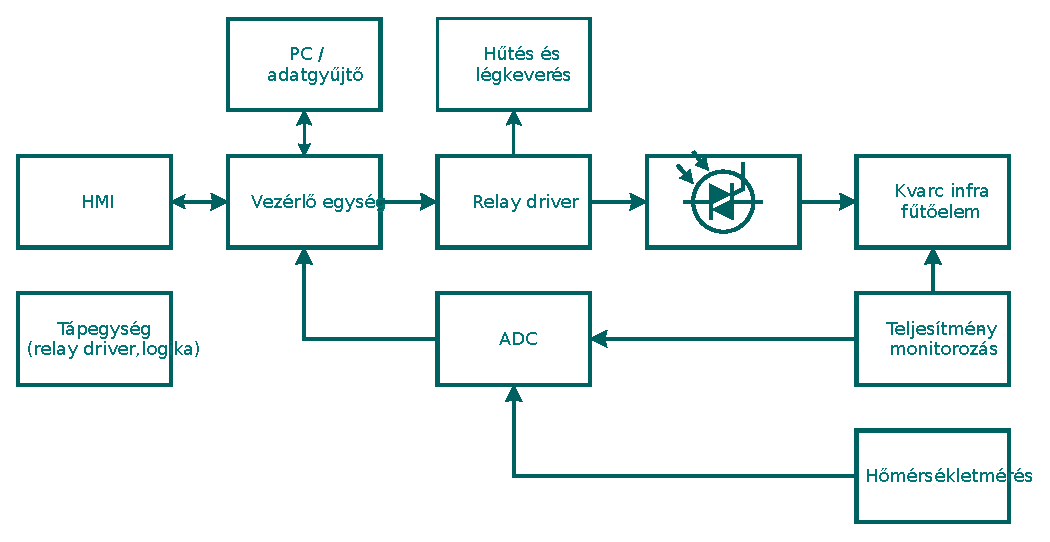
\includegraphics[width=0.9\textwidth]{spec_v10}
 \caption{Rendszerarchitektúra az előzetes specifikáció alapján}
\end{figure}



\end{document}
